Our \textit{dynamic programming} algorithm:
\begin{itemize}
  \item By using \textit{depth-first} search(choosing an arbitrary node as a root), we calculate three arrays:
  \begin{itemize}
    \item $d1[i]$: minimum sum achievable by only using node $i$ and its descendants.
    \item $p[i]$: predecessor of node $i$ in the path found for $d1[i]$.
    \item $d2[i]$: second minimum sum achievable by only using node i and its descendants, a path that is edge-disjoint relative to the path found for $d1[i]$. 
  \end{itemize}
  \item When we calculate these arrays, we can get the overall minimum sum by\\ $\min(d1[k], d2[k], d1[k] + d2[k])$ over all nodes $k$ because path can be in two shapes:
  \begin{itemize}
    \item Straight path from node $k$ to its descendants or bend over at node $k$:
       \begin{figure}[ht]
        \centering
        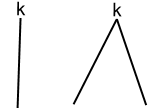
\includegraphics[width=0.2\textwidth]{q2}
        \caption{Basic shapes of the minimum path}
    \end{figure}
  \end{itemize}
  \item Calculation of $d1[i]$:
  \begin{itemize}
    \item Run a depth-first search from the root node(chosen arbitrarily). In the DFS, keep track of the current node and its predecessor. At each node, assume its children are $n_1, n_2, \dots n_k$. Then, $d1[i] = \min(\min(d1[n_1] + cost[i, n_1], d1[n_2] + cost[i, n_2], \dots, d1[n_k] + cost[i, n_k]), \min(cost[i, n_k]))$. Also note that, $d1[i]$ is set to 0 if node $i$ is a leaf. Moreover, we update $p[i]$ with the selected predecessor to retrieve the path later.
  \end{itemize}
  \item Calculation of $d2[i]$:
  \begin{itemize}
    \item Run a depth-first search from the root node(chosen arbitrarily which is same node used in $d1[i]$ calculations). Apply the same logic we did for $d1[i]$, except when going from a node $i$ to one of its children $k$, update $d2[i]$ only if $p1[i] \neq k$. We do this for all children recursively.
    \item $d2[i] = \min(d2[i], d1[k] + cost[i, k], cost[i, k])$ where node $k$ is the children of node $i$.
  \end{itemize}
\end{itemize}

We call depth-first twice, which is linear, to calculate $d1[i], d2[i]$ and $p[i]$ arrays. We also go over of all vertices again to take the minimum sum by possible $d1[i], d2[i]$ or merge of both. Therefore, overall complexity remains \textit{linear}.